\part{Exigences scientifiques et pérennisation de l'IA}

%%%%%%%%%%%%%%%%%%%%%%%%%%%%%%%%%%%%%%%%%%%%%%%%%%%%%%%%%%%%%%%%%%%%%%%%%%%%%%%%%%%%
%%%%%%%%%%%%%%%%%%%%%%%%%%%%%%%%%%%%%%%%%%%%%%%%%%%%%%%%%%%%%%%%%%%%%%%%%%%%%%%%%%%%
%%%%%%%%%%%%%%%%%%%%%%%%%%%%%%%%%%%%%%CHAPITRE%%%%%%%%%%%%%%%%%%%%%%%%%%%%%%%%%%%%%%
%%%%%%%%%%%%%%%%%%%%%%%%%%%%%%%%%%%%%%%%%%%%%%%%%%%%%%%%%%%%%%%%%%%%%%%%%%%%%%%%%%%%
%%%%%%%%%%%%%%%%%%%%%%%%%%%%%%%%%%%%%%%%%%%%%%%%%%%%%%%%%%%%%%%%%%%%%%%%%%%%%%%%%%%%

\chapter{Familiarisation avec l'IA et limitations identifiées}

Au sein de cette partie nous voulons revenir sur le travail et les observations menées au sein même des équipes. Nous venons d'aborder le résultat des prises en main d'outils entre juillet et août 2025, mais le travail d'introduction et de formation à l'IA est un travail au long cours qui a été entamé dès le début de la collaboration entre le MAD et l'École des Chartes. 

\section{Enthousiasmes et réticences face à l'automatisation}

Dans le cadre des missions des musées labellisés "Musée de France", le musée des Arts décoratifs a pour mission de \enquote{Conserver, restaurer, étudier et enrichir [ses] collections}\footnote{\cite{noauthor_loi_2002}}. Cela implique entre autre la bonne tenue et documentation d'un inventaire des œuvres. Cette tâche, peut-être plus que celles concernées par l'automatisation, est souvent le point d'entrée par lequel les équipes abordent la perspective de l'introduction de l'IA dans leur travail. Nous allons donc détailler dans ce qui suit, le chemin parcouru et les éventuelles réticences soulevées par les employé\wokisme e\wokisme s au contact de l'IA.

\subsection{Le travail de pédagogie et de présentation}

Depuis le lancement du projet Royère il y a trois ans, un long travail d'expérimentation et de formation a été entamé au musée des Arts décoratifs, et pas seulement au département des Arts graphiques. Marion Charpier a formé les personnels et présenté des outils et des méthodes nouvelles à plusieurs équipes, tout en restant à l'écoute des besoins. Elle est notamment intervenue auprès du Service Informatique et de la gestionnaire de la base de données en plus du département des Arts graphiques. Ce travail de fond, d'acculturation des équipes et de vulgarisation de l'intelligence artificielle et de ses capacités à été crucial. En effet, tous les projets que nous pourrions formuler, ou qui pourraient être mis en place courent le risque de ne pas être utilisés ou de devenir accessoires, si les équipes ne s'en emparent pas. L'autre aspect est aussi que les agents ne doivent pas se sentir remplacés ou diminués par l'introduction de l'IA dans les processus de travail. C'est pourquoi le travail d'explicitation et de vulgarisation est primordial afin de montrer les limites et potentialités d'un outil d'IA.

Ces enjeux de présentation se sont poursuivis lors de notre présence au musée, que ce soit par la présentation que nous avons co-animée avec Marion Charpier et Emmanuelle Bermès face aux employés et à la direction le 24 avril 2025, ou bien par la campagne d'entretiens que nous avons menée, dans la droite lignée du travail entamé par Marion Charpier. En effet, deux ans après le début de la collaboration entre l'École des Chartes et le MAD, elle a mené une première campagne d'entretiens sur l'impact potentiel que pourrait avoir l'IA et son introduction au musée. Nous joignons ici ses conclusions et interrogations, avec ce que nous avons pu nous-même recueillir ou observer à propos des pratiques et conceptions autour de l'IA plusieurs mois après.

\subsection{Les leçons des entretiens et l'applicabilité de l'IA}

Dans la série d'entretiens menés en décembre 2024, plusieurs cas d'usages apparaissent. Il y a deux grands domaines dans lesquels l'introduction de l'IA pourrait être très utile : l'inventaire et l'exploration visuelle des collections. En ce qui concerne l'inventaire, l'IA pourrait faciliter l'indexation des œuvres et la gestion des archives historiques, en proposant des pré-indexations et de courtes descriptions sommaires afin d'attribuer des mots-clefs pertinents. Emmanuelle Bermès et Marion Charpier notent sur ce point :\enquote{Une autre possibilité réside aussi dans la création automatique de fiches d'inventaires, permettant d'attribuer systématiquement un numéro à chaque œuvre et de réduire le temps consacré aux tâches administratives}\footnote{\cite{bermes_repenser_2025}. p. 5.}. Pour les archives historiques, l'IA pourrait faciliter le traitement des numérisations et permettre l'amélioration des connaissances sur les œuvres, notamment en utilisant de l'HTR et du NER afin de croiser les informations et d'extraire les noms de personnes, lieux, organisations, etc,. mentionnés.

Pour l'exploration visuelle des collections, \enquote{l'IA pourrait considérablement enrichir l'exploration des collections en facilitant l'identification d’œuvres similaires, en optimisant la gestion des médias et en assistant les équipes dans leurs recherches de provenance}\footnote{\cite{bermes_repenser_2025}. p. 5.}. Il y a un vrai intérêt pour l'optimisation de la gestion des collections, mais cela implique plusieurs choses : \enquote{garantir la fiabilité des résultats, éviter les biais dans l'indexation, protéger la confidentialité des informations et s'assurer que les infrastructures techniques puissent supporter l'augmentation du volume de données traitées}\footnote{\cite{bermes_repenser_2025}. p. 5.}. En effet, la particularité des collections du MAD fait que beaucoup des œuvres présentes sont encore sous droits au profit de maisons ou de particuliers et que la libre diffusion de ces matériaux n'est pas possible. Il faut donc s'assurer que les traitements que nous mettons en place ne risquent pas de mettre entre les mains d'un tiers des données protégées ou sensibles. Un autre aspect qui ressort et qui invite à la prudence est le poids et le coût des numérisations. On estime que seul 30\% des collections sont numérisées, et bien que toutes les personnes que nous avons interrogées, pendant les entretiens de juillet-août 2025, citent que de nombreux fonds pourraient bénéficier de numérisations ou de traitements IA, toutes invitent à la prudence et préviennent que de trop grands volumes à traiter d'un coup seraient délétères pour la qualité et la faisabilité de leur travail quotidien. Enfin, la plupart des personnes disent être prêtes à consacrer du temps à la relecture ou correction de données générées, si cela permet d'aller plus vite que l'option manuelle, mais elles signalent aussi exiger une certaine qualité dans les données proposées. Tous\wokisme tes acceptent une marge d'erreur, tant qu'elle n'est pas inférieure à celle que pourrait faire un humain face à la même tâche, notamment pour les missions sensibles comme l'inventaire et l'indexation.

Afin de résumer, en reprenant la synthèse des entretiens de décembre 2024, le cadre d'application et l'impact de l'IA dessiné par les acteurs au fil des entretiens tient en cinq points fondamentaux. Il faut que l'IA soit appliquée dans un cadre sécurisé qui permette de garder le contrôle sur les enjeux de confidentialité et de contrôle des données sensibles. Il y a une grande motivation à appliquer l'IA afin de pouvoir traiter le volume important de passifs accumulés, que ce soit dans la base de données, l'inventaire ou la gestion des collections. L'utilisation de l'IA doit se faire dans un cadre strictement régulé, avec une tolérance partielle aux erreurs, des démarches de contrôle qualité par échantillonnage et des processus de validation sous la responsabilités des personnels scientifiques. L'absence de mise en œuvre de l'IA aurait pour conséquence de maintenir les délais actuels, parfois trop long, pour certaines tâches essentielles. Enfin, les erreurs produites par l'IA auraient un impact modéré, se traduisant principalement par des perturbations gérables dans le travail quotidien grâce à une supervision humaine régulière et à une attention particulière au volume de données générées pour ne pas submerger les personnels.

Parmi les personnes que nous avons pu interroger ou que Marion Charpier a interrogé, la plupart semblent enthousiaste à l'introduction de l'IA, mais il ne faut pas s'y tromper. Il y a bel et bien un intérêt et une volonté d'adopter l'IA au sein du musée, mais cet intérêt \enquote{repose avant tout sur la recherche d'une solution viable aux défis liés au traitement des collections. Plus que l'IA en tant que telle, c'est avant tout une réponse efficace au passif à traiter qui suscite l'intérêt des acteurs du musée}\footnote{\cite{bermes_repenser_2025}. p. 6.}. Il ne faut pas oublier non plus qu'il peut exister au sein du musée un ressentiment ou une crainte vis-à-vis de ce genre de projets. L'IA ne fait pas l'unanimité, certain\wokisme e\wokisme s redoutent d'être remplacé\wokisme e\wokisme s. Cela évoque des peurs, ou des griefs lorsque des budgets sont alloués à cela et pas à d'autres activités dans le musée, comme des restaurations ou des embauches. C'est en gardant tout cela à l'esprit que le déploiement d'un ou plusieurs projets IA doit se faire. 

Enfin, le grand absent de ces entretiens et expérimentations reste tout de même la photothèque du musée. Les projets Royère et TORNE-H s'articulant autour des collections d'arts graphiques, il est normal que l'attention se soit portée sur ce département. Cependant, au fur et à mesure de notre stage, il est apparu, de manière très claire, au gré des interactions informelles avec l'équipe de la photothèque, ou à travers certaines remarques des personnels de conservation du département des Arts graphiques, que l'équipe de la photothèque aurait aussi largement besoin d'outils pour faciliter leur travail. L'équipe a sous sa responsabilité toutes les ressources photographiques et numérisées du musée et semble effectivement être une cible de choix pour l'introduction d'outils de reconnaissance par similarité, ou de \textit{computer vision} pour leur permettre un traitement massif et structuré de ces données. 

\section{Des projets IA et des hommes}

Nous avons parlé de projets mobilisant l'IA, au sein des musées, des institutions patrimoniales ou d'entreprises, et nous mobilisons cette notion lorsque nous évoquons le projet Royère et TORNE-H, mais nous devons préciser deux distinctions fondamentales pour la suite de notre raisonnement. Tous les projets IA n'utilisent pas la même logique. Cela revient à ce que nous évoquions en Introduction lorsque nous distinguions entre IA connexionniste et IA symbolique, mais tous les projets IA n'utilisent pas les mêmes mécanismes. l'IA générative, la plus connue, celle des ChatGPT et autres agents conversationnels, se fonde sur les principes connexionnistes et offre une grande plasticité du fait de ses connaissances généralistes. Cependant, en dépit de sa facilité d'introduction dans un processus, de par l'absence de pré-configuration nécessaire, elle est celle qui rencontre le plus d'écueils dans des projets scientifiques, car sujette aux hallucinations et peu sûre en terme de confidentialité de données. De l'autre côté l'IA analytique génère des données structurées, est faite pour la catégorisation, la prédiction ou l'extraction de données et se base sur des algorithmes de machine learning pour accomplir sa tâche. Le projet TORNE-H, par exemple, se situe dans cette dernière catégorie. C'est la raison pour laquelle il est important de revenir sur quelques points d'attention et quelques exemples de projets passés ou présents qui peuvent nous en apprendre beaucoup sur les manières d'introduire ou non l'IA dans les domaines du patrimoine.

\subsection{Projets \textit{Venice Time Machine} et HikarIA}

Nous voulons vous présenter ici deux projets, l'un en cours, l'autre suspendu, afin de tenter de tirer les leçons de ces expériences dans le domaine patrimonial. Tout d'abord, un projet européen initié par l'université Ca'Foscari de Venise et l'École Polytechnique Fédérale de Lausanne (EPFL) en 2013 et concrétisé avec la signature d'un \textit{Memorandum Of Understanding} entre l'université, l'EPFL et les archives d'État de Venise en décembre 2014\footnote{\cite{castelvecchi_venice_2019}}. Le projet voulait reconstruire 1000 ans d'histoire de la cité à travers ses archives, leur numérisation et le recoupement avec les sources iconographiques et photographiques de la ville\footnote{\cite{epfl_presentation_2017}}. Le projet couplait HTR, NER, entraînement de modèle d'IA et numérisation massive des archives de la ville\footnote{\textit{cf}. le \textbf{\hyperref[sec:Glossaire]{Glossaire}} pour les termes \enquote{HTR} et \enquote{NER}, p.~\pageref{sec:Glossaire}.}. L'ambition était de mettre à disposition des historien\wokisme nes, des données massives et interrogeables afin de faire l'histoire sociale, politique et architecturale de Venise. Cependant, il semble que plusieurs problèmes aient mené à la suspension du projet, le 19 septembre 2019 par les archives d'État de Venise\footnote{\cite{noauthor_sospensione_nodate}}. Dans le communiqué, l'institution cite une absence de méthodes de travail uniforme, de norme de partage de données, une absence de communication entre les institutions, un manque d'équité, et une absence d'accord autour de la divulgation des données et des droits. En cinq ans, plus de 190 000 documents ont été numérisés, générant près de 8 TB de données\footnote{\cite{burns_venice_2019}}. Il semblerait que les deux problèmes principaux aient été les formats et l'absence de documentation idoine des numérisations qui auraient dû répondre aux exigences de la norme InterPARES utilisée par les archives d'État de Venise, et l'absence de communication entre les institutions\footnote{\cite{castelvecchi_venice_2019}}. Le second problème ayant causé le premier, les données générées se retrouvent inutilisables pour les archives en plus d'avoir été manipulées et gérées de manière opaque par l'EPFL. 

Ce que nous dit ce projet impressionnant mais malheureusement reporté \textit{sine die}, faute d'accord, est que dans les projets de numérisation et de traitement automatique la pleine transparence et maîtrise du processus par tous les acteurs est fondamentale. Pour notre cas ce ne sont pas plusieurs institutions étrangères qui doivent communiquer, mais l'incompréhension et le manque de transparence peut aussi très bien advenir entre des services ou entre une institution et un prestataire. C'est pour cette raison que le travail de pédagogie, de cadrage des besoins, d'explicitation des procédés, d'accord sur la forme des rendus finaux est primordial et doit être accompagné par des réunions de consultation et des points de passages concertés sur les projets, pouvant être inspirés des méthodes Agiles\footnote{\textit{cf}. le \textbf{\hyperref[sec:Glossaire]{Glossaire}}, p.~\pageref{sec:Glossaire}.}. 

Puis, le second projet, qui court jusqu'en 2026, est une collaboration entre l'entreprise Teklia et le musée Guimet à Paris. Il est soutenu par l’État dans le cadre du dispositif \enquote{Numérisation du patrimoine et de l’architecture} de France 2030, opéré par la Caisse des Dépôts\footnote{\cite{noauthor_projet_nodate}}. Le projet porté par Christopher Kermorvant, PDG de Teklia et Édouard de Saint-Ours, conservateur des collections photographiques au Musée Guimet a pour but d'entraîner \enquote{des algorithmes d’intelligence artificielle [...] à reconnaître des éléments visuels dans un vaste corpus produit entre le milieu du \textsc{xix}\textsuperscript{e}~siècle et le début du \textsc{xx}\textsuperscript{e}~siècle[...]. Ces algorithmes seront mis en œuvre sur une plateforme d’analyse qui feront émerger du corpus des données statistiques inédites sur les palettes de couleurs, les séquences d’images, les constantes et les ruptures iconographiques (doublons, lieux, décors, accessoires, modèles, typologies)}\footnote{\cite{noauthor_projet_nodate}}. Il y a deux volets au projet, une partie découpage automatisé des images dans les albums avec un entraînement de modèle d'extraction de photographie, qui semble avoir donné des résultats très satisfaisants. Le résultat de ces extractions sont les nombreuses vues disponibles sur le site du projet\footnote{\cite{noauthor_hikaria_nodate-1}}. De plus, la présentation des vues propose un système de \textit{clustering} par similarité, très proche des technologies que nous avons expérimentées dans le stage, qui propose des images que l'algorithme juge similaires à celle que nous regardons en bas de page.

L'autre volet, qui semble avoir été abandonné depuis la version 0.2.6 du projet, mais qui était encore présent dans la version 0.2.5, était la génération de mots-clefs et de descriptions automatiques par un LLM afin d'enrichir les métadonnées et les descriptions. En effet, quand nous avions inspecté les résultats générés sur la dixième vue de l'album 47 du fonds Dubois, on pouvait voir tant des mots-clefs établis par le documentaliste que ceux générés par IA\footnote{\cite{noauthor_hikaria_nodate}}. La photographie montre deux femmes portant des ombrelles devant un portail en bois menant à une maison. Si le grand modèle de langue avait relevé quelques termes pertinents non indexés par le documentaliste, notamment \enquote{barrière}, \enquote{portail} ou \enquote{chemin}, beaucoup de termes générés sont faux ou non pertinents, comme \enquote{bac à gaz}, \enquote{punition}, \enquote{consulat} ou, de manière plus problématique, \enquote{Chine}. Depuis, ces descriptions automatiques ont été enlevées du site et notre seule source est le travail de rédaction de Pierre Husson dans le cadre de son stage à l'INHA, qui a rédigé une partie sur le projet avant sa mise à jour, fin août, et qui nous permet de sourcer ce que nous avions vu à l'époque sans le prendre en capture d'écran ou l'archiver. 

On comprend néanmoins pourquoi ce volet du projet, pourtant si prometteur, a été retiré (peut-être seulement temporairement). Du point de vue d'un conservateur, des photographies japonaises du \textsc{xix}\textsuperscript{e}~siècle, qui se retrouvent affublées d'une description \enquote{Chine} est intolérable, et à raison . L'ancrage culturel des modèles d'IA dans des perspectives culturelles occidentales, explique l'erreur : les données d'entraînement comprennent des biais culturels, qui sont reproduits dans les analyses produites. Le projet a encore un an devant lui, et il est doté d'un corpus numériquement similaire au nôtre avec le projet Royère (environ 18 000 photos). Beaucoup de choses peuvent encore changer, et être affinées mais il nous semble que cela nous invite à deux constats importants pour nous. D'abord, la notion de marge d'erreur ne comprend pas du tout les mêmes types de problèmes que lorsque l'on parle de marge d'erreur dans le travail humain de récolement et de description. Dans les entretiens menés par Marion Charpier, il apparaît que les personnels sont prêts à accepter une certaine marge d'erreur, en vertu de la probabilité similaire qu'il existe des erreurs dans le travail humain. Cependant, du point de vue scientifique, le type d'erreur que peut générer un traitement automatisé n'est pas du tout de même nature qu'un oubli ou une erreur d'interprétation, qui elles auront toujours bien plus le contexte à l'esprit. Un LLM malheureusement est aussi emprunt de biais, tout comme les humains qui l'ont construit ou les données sur lesquelles il a été entraîné. Ce qui nous fait arriver à notre second constat : la méfiance nécessaire vis-à-vis des données générées par une IA générative de type Chat-GPT, Claude, Mistral, Deepseek, etc,. Ces modèles sont par nature des modèles probabilistes, ils génèrent en fonction de la plus ou moins haute probabilité que le mot \textit{N} suive le mot \textit{N-1} et fasse sens dans le contexte qu'il comprend via ses embeddings\footnote{\textit{cf}. le \textbf{\hyperref[sec:Glossaire]{Glossaire}}, p.~\pageref{sec:Glossaire}.}. La nature généraliste et biaisée de ces modèles invite donc à la plus grande méfiance et retenue dans leur utilisation pour des collections patrimoniales, imposant, par exemple, l'utilisation d'un vocabulaire contrôlé ou d'une ontologie fixe pour les générations, un peu à la manière de l'inférence Royère.

\subsection{Points d'attentions et moyens humains}

Dans ces projets et dans d'autres qui pourraient exister au sein du musée des Arts décoratifs ou ailleurs, il est crucial de garder à l'esprit deux choses pour la pérennité des résultats des traitements automatisés : les cas d'usages et le coût humain de la numérisation ou de l'automatisation. Le premier point est d'autant plus crucial que \enquote{réussir un projet IA, c’est avant tout répondre aux besoins des équipes terrain. Ce qui signifie, identifier avec précision l’usage futur de l’IA au sein de l’organisation afin de définir des choix technologiques, de structurer l’allocation de ressources et de s’atteler à un sujet conséquent : la préparation des données}\footnote{\cite{it_social_ia_2025}}. Nous prenons cette citation d'un magazine technologique destiné aux entreprises et qui parle des entreprises, mais il nous semble cependant qu'une partie des conclusions qu'ils tirent sur l'introduction de l'IA en entreprise, soient applicables dans notre cas. En effet, l'article cite le taux d'échec élevé des projets IA en entreprise (85\%), et bien que nous soyons bien incapables de donner une statistique similaire dans le milieu du patrimoine et des humanités numériques, il n'empêche que les raisons évoquées sont éloquentes à plusieurs égards : 
\vspace{1em}

\noindent
\hspace*{1cm}
\begin{minipage}{\dimexpr\linewidth-2cm}
\fontsize{10}{12}\selectfont
Les entreprises manquent fondamentalement d’expérience et de recul[...] Un des premiers indices de cette non-maturité est structurel. Sans expérience ni méthode, un grand nombre d’entreprises tendent à créer des couches organisationnelles redondantes. Il est ainsi fréquent de voir émerger des départements spécialisés IA en supplément de départements existants dédié à l’innovation ou à l’informatique.\footnotemark{}
\end{minipage}

\vspace{1em}

\footnotetext{{\cite{it_social_ia_2025}}} 

Le second point fait référence à l'effort consenti et conscientisé par l'institution pour intégrer durablement les données ou numérisations produites. Dans le cas des numérisations, le problème n'est pas nouveau, mais il fonctionne de manière similaire. 


\vspace{1em}

\noindent
\hspace*{1cm}
\begin{minipage}{\dimexpr\linewidth-2cm}
\fontsize{10}{12}\selectfont
De nombreux projets de numérisations, ont fleuri il y a quelques années, à la faveur de financements en ce sens. Nous nous sommes retrouvés avec quantité d'images, qui sont restées là sur des disques dur ou des drives, dont on a perdu la trace ou qui n'ont pas survécu au passage dans la base de donnée commune des musées en 2015. Certes, certaines campagnes de numérisations sont redécouvertes par la suite, mais la plupart du temps, nous les responsables des collections, n'avons pas le temps d'accomplir ce travail de fond de caractérisation et d'intégration, pourtant nécessaire. \footnotemark{}
\end{minipage}

\vspace{1em}

\footnotetext{Propos recueillis auprès de Sébastien Quéquet, attaché de conservation en charge des collections de photographie au MAD, le 12 août 2025.} 

Le point sur lequel appuyait Sébastien Quéquet lors de notre entretien est celui du manque de main-d’œuvre pour absorber et intégrer durablement, notamment dans la base Arcadie, les informations et les représentations des œuvres. Il cite évidemment l'embauche de stagiaires ou de contrats courts pour réaliser cette tâche, mais cela peut s'avérer compliqué lorsque l'on sait que les postes ponctuels comme ceux-là, sont conditionnés le plus souvent à l'obtention d'un mécénat. C'est pour cela qu'il évoquait la nécessité de penser en amont, dans la création et le financement d'un projet, à l'embauche des personnes qui pourraient faire ces intégrations. 

Une autre piste évoquée à ce moment-là, et qui est déjà fort répandue dans le monde des archives, est l'indexation collaborative. Il s'agit de campagnes ouvertes au publics, organisées par les archives départementales de nombreuses localités, qui ont pour but de mettre à disposition des numérisations d'archives, d'une même source (par exemple archives ecclésiastiques ou notariales) et de les faire annoter par les érudits locaux et les passionnés d'histoire de la région afin de faciliter le travail des archivistes. La plateforme qui réunit ces initiatives pour les Archives Nationales se nomme Girophares et a été lancée en 2023\footnote{\cite{noauthor_archives_nodate}}. Il existe aussi de nombreuses archives départementales comme celles de Haute-Garonne, du Calvados, du Bas-Rhin, de l'Oise, du Cantal et bien d'autres qui disposent d'interfaces similaires. Ce qui nous fait dire que l'option n'est pas si fantasque, est qu'un premier essai en musée a déjà eu lieu au Musée de Bretagne\footnote{\cite{noauthor_lindexation_nodate}}. En 2020, accompagné par la Bnf, la société Teklia, la société Decalog et dans le cadre d’un appel à projet à services numériques innovants, lancé par le ministère de la Culture, le musée lance sa plateforme pour indexer ses fonds photographiques.

Ce qu'il s'agit ici de démontrer est que le besoin doit toujours présider au développement d'une solution. Cette solution doit s'intégrer dans les habitudes et le travail des équipes, sans causer de doublons ou de redondances organisationnelles. Les possibilités de l'IA peuvent effectivement déclencher un effet d'attraction, mais il faut toujours réfléchir en amont aux résultats attendus ou recherchés et à la mise en place d'un environnement de données adéquat\footnote{À cet effet le guide produit par la \textit{Library of Congress} nous semble très éclairant à plusieurs égards : \cite{manchester_introducing_2023}}. Enfin, les logiques de projet doivent inclure dans leur calendrier et leur budget les moyens de la pérennisation de ces productions, que ce soit par des équipes de suivis ou le personnel scientifique nécessaire à la pleine intégration des informations dans les corpus du musée.

%%%%%%%%%%%%%%%%%%%%%%%%%%%%%%%%%%%%%%%%%%%%%%%%%%%%%%%%%%%%%%%%%%%%%%%%%%%%%%%%%%%%
%%%%%%%%%%%%%%%%%%%%%%%%%%%%%%%%%%%%%%%%%%%%%%%%%%%%%%%%%%%%%%%%%%%%%%%%%%%%%%%%%%%%
%%%%%%%%%%%%%%%%%%%%%%%%%%%%%%%%%%%%%%CHAPITRE%%%%%%%%%%%%%%%%%%%%%%%%%%%%%%%%%%%%%%
%%%%%%%%%%%%%%%%%%%%%%%%%%%%%%%%%%%%%%%%%%%%%%%%%%%%%%%%%%%%%%%%%%%%%%%%%%%%%%%%%%%%
%%%%%%%%%%%%%%%%%%%%%%%%%%%%%%%%%%%%%%%%%%%%%%%%%%%%%%%%%%%%%%%%%%%%%%%%%%%%%%%%%%%%

\chapter{La \textit{computer vision} au musée en puissance et en acte}	

Fort des connaissances sur les possibilités offertes par la recherche actuelle en humanités numériques, et conscient de l'histoire et de la particularité du musée des Arts décoratifs et de l'Union Centrale plus largement, nous nous proposons de dresser un premier bilan et un premier tableau prospectif de l'introduction de l'IA dans l'institution.

\section{MLOps et compétences techniques nécessaires}

L'un des enjeux du projet Royère puis du projet TORNE-H, était la formation des équipes aux notions fondamentales de l'IA. L'un des aspects de cette formation que nous n'avons pas encore évoqué était celle à destination du Service Informatique du musée. En effet, de par leur rôle, tout projet d'automatisation ou de \textit{Machine learning} devait aussi être réfléchi avec le service pour qu'il puisse être mis en place. C’est pourquoi Marion Charpier a assuré un certain nombre de formations sur les fondamentaux de l'IA et de son environnement auprès du SI. Les équipes du SI, curieuses d'apprendre, se sont prêtées au jeu et ont fait tout ce qui était en leur pouvoir afin de mettre en place un environnement de développement, comme nous l'évoquions dans une partie précédente. Elles ont aussi participé aux discussions autour de la conception des flux de données et ont veillés à la sécurisation des matériaux dans le cadre du projet Royère. 

Dans ce cadre, plusieurs journées de bilan, formation et ateliers ont eu lieu pendant le stage. S'est tenu un atelier de cartographie des compétences nécessaires pour la mise en place d'une opération de \textit{Machine learning}. Une intervention de la part de la Fondation SAHAR, dans le cadre d'un mécénat de compétences, pour nous introduire au DevOps et au rôle d'un \textit{Data Scientist}, et enfin une formation à Docker et à la conteneurisation d'application par un enseignant de l'École\footnote{\textit{cf}. le \textbf{\hyperref[sec:Glossaire]{Glossaire}} pour le terme \enquote{\textit{Data Scientist}}, p.~\pageref{sec:Glossaire}.}. Ces initiatives ont permis de mettre en lumière le chemin qu'il restait à parcourir avant la mise en production pérenne d'une opération de \textit{Machine learning}, mais aussi la capacité d'adaptation et la volonté d'apprendre des équipes du musée.

\subsection{Décrire une chaîne IA}

Afin de bien comprendre de quoi il retourne lorsque nous parlons de la mise en production d'une opération de \textit{Machine learning}, nous revenons ici très généralement sur la manière dont se construit une chaîne de production MLOps, puis plus précisément sur son applicabilité dans le domaine patrimonial. Nous nous appuyons sur un article de recherche généraliste et orienté vers l'application d'un MLOps dans le secteur privé pour donner un aperçu des grandes questions et enjeux qui parcourent l'élaboration et la mise en production d'un projet de \textit{machine learning}\footnote{\cite{kreuzberger_machine_2023}}. 

\begin{figure}[H]
    \centering
    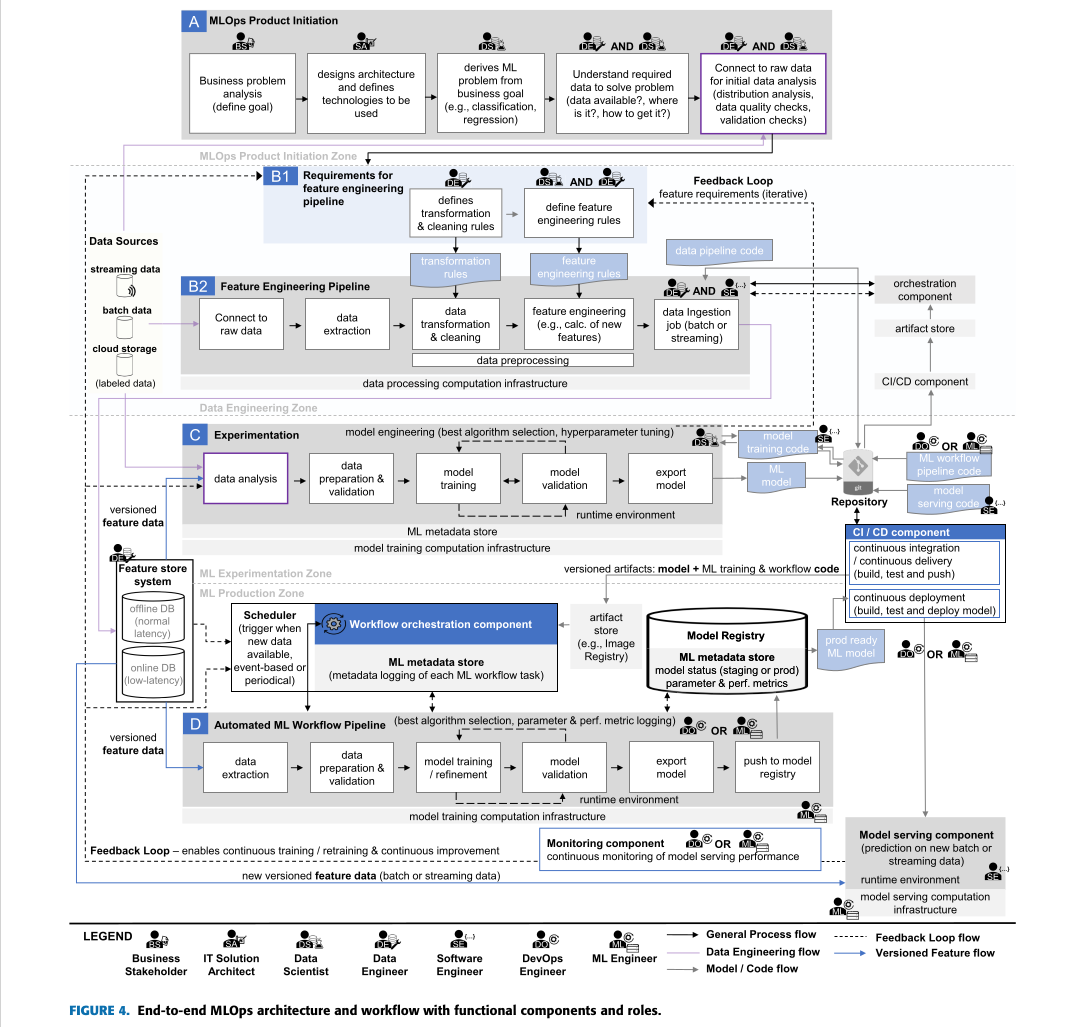
\includegraphics[width=1.08\linewidth]{Illustrations/MLOps.png}
    \caption{Schéma d'une architecture de MLOps}
    \label{fig:placeholder}
\end{figure}

Si nous reprenons le modèle exposé dans ce schéma, très complet et complexe, on voit plusieurs choses\footnote{\cite{kreuzberger_machine_2023}. p. 31873}. Il comprend quatre grandes étapes : l'initiation du projet, la conception des \textit{features}, l'expérimentation et la mise en production. Ce que nous devons garder à l'esprit est la diversité des compétences requises pour mener à bien un tel processus. Entre les personnes métiers qui prennent part au processus, les ingénieurs logiciel, DevOps, \textit{Data} et \textit{Machine learning}, un \textit{Data Scientist}, un \textit{Data engineer} et un \textit{IT Solution Architect}, beaucoup de corps de métiers entrelacés sont convoqués. Dans l'exemple donné, le schéma est appliqué à un produit commercialisable, et dans les ambitions d'un musée, une équipe aussi nombreuse ne serait sans doute pas pertinente. Cela demande tout de même que les personnes aient des compétences hybrides et transversales et qu'une certaine expérience de l'industrialisation et de la gestion de flux de données soit présente.

Aussi, il faut garder à l'esprit que l'histoire de l'art se prête assez mal aux traitements quantitatifs. C'est la raison pour laquelle Marion Charpier a dû utiliser un algorithme de déformation d'images pour enrichir le jeu de données dans son \textit{workflow} TiamaT.

\vspace{1em}
\noindent
\hspace*{1cm}
\begin{minipage}{\dimexpr\linewidth-2cm}
\fontsize{10}{12}\selectfont
While museum datasets are not complete enough to train algorithms potentially museums could work together to produce an algorithm that could be applied in the sector. There is also an opportunity for museums to partner with the data science community to create machine learning models based on smaller datasets specifically for art objects.                                                  \footnotemark{}
\end{minipage}
\vspace{1em}
\footnotetext{\cite{murphy_museum_2020}. p. 9.}

Ce sont toutes ces questions qui ont mené le projet TORNE-H à s'orienter vers une démarche résolument qualitative en privilégiant l'apprentissage supervisé à l'apprentissage machine. Nous voulons partager un extrait d'un livre collectif publié en 2010, qui illustre assez bien les questions qui se posent aujourd'hui en histoire de l'art et traitement patrimonial en lien avec l'IA : 

\vspace{1em}
\noindent
\hspace*{1cm}
\begin{minipage}{\dimexpr\linewidth-2cm}
\fontsize{10}{12}\selectfont
Pourquoi les statistiques, les graphiques et les cartes ne sont-ils pas aimés en histoire de l’art ? Les approches quantitatives dans ce domaine, souvent importées de la sociologie, portent probablement la macule de la discipline de Durkheim : réductionnisme, incapacité à rendre compte des œuvres, approche centrée sur les stratégies, le marché, l’argent, le collectif et la norme, alors que l’art et la création sont inséparables du désintéressement, des sacrifices, de l’individualité, du génie, et que le rôle de l’historien de l’art est de reconstituer des styles, de rendre compte de la valeur de l’art et des œuvres exceptionnelles.                                                \footnotemark{}
\end{minipage}
\vspace{1em}
\footnotetext{\cite{joyeux-prunel_lart_2010}. p. 17.}

Tout cela a été écrit en 2010, plusieurs années avant l'émergence des première réflexions autour de l'intelligence artificielle et de l'histoire de l'art. Cela n'empêche pas que, pour nous, nous retrouvions les mêmes problématiques, les mêmes tensions entre sciences idiographiques et sciences nomothétiques, que celles qui ont traversé les réflexions en histoire et sociologie par rapport à l'émergence au \textsc{xx}\textsuperscript{e}~siècle du quantitativisme. Les démarches statistiques fondées sur les grands ensembles de données et la répétition, qui sont l'apanage des modèles d'intelligence artificielle, ne sont pas toujours compatibles avec la particularité des fonds ou la singularité des oeuvres. C'est cette tension que l'on doit aussi garder à l'esprit pendant l'élaboration d'un projet de \textit{machine learning} dans une institution patrimoniale. En d'autres termes : que peut-on attendre, ou que ne faut-il pas attendre d'un traitement par IA sur des collections patrimoniales ?

\subsection{Le traitement Royère et le projet TORNE-H}

La tentative d'introduction d'un processus de \textit{machine learning} nous a permis de cadrer les besoins et d'explorer les possibilités et limites de cette démarche. Avant l'opérationnalisation d'un traitement IA, plusieurs étapes sont fondamentales. Nous l'avons déjà détaillé : le recueil des besoins, l'étude de l'état des données, des collections et de l'infrastructure existantes, le diagnostic des compétences et la marge d'évolution possible des personnels et infrastructures. Toutes ces composantes interviennent avant même le traitement IA à proprement parler. Pour ce qu'il en est du processus en lui-même, et de ce que nous pouvons généraliser à partir de ces deux projets, Royère et TORNE-H, nous pouvons dire deux choses. D'abord il y a un intérêt réel, tant du point de vue scientifique, que du point de vue des équipes, pour l'introduction de ce genre de traitement, et les bons résultats de l'inférence Royère nous font dire que la démarche de \textit{fine-tuning} porte ses fruits et est pleinement justifiée dans le cadre des collections patrimoniales. Cependant, nous avons du mal à amener la précision et le détail d'analyse que les équipes souhaiteraient. Nous avons pu caractériser ce qu'il se trouvait sur les 12 000 images, mais pas les motifs ou les modèles de meubles, ce qui aurait vraiment été une valeur ajoutée pour les personnels en charge des collections. Ensuite, outre les limitations techniques de puissance de calcul, la base de données Arcadie n'est pas en mesure d'absorber de grandes quantités de notices à la fois sans risque de crash. Nous sommes limités à des lots de 10 GB de médias à la fois et quand il s'agit d'une collection de 12 000 images, cela peut s'avérer très compliqué. La tâche est d'autant plus complexe que les imports doivent se faire sur les heures de travail et au prix d'un ralentissement de la base pour tous les autres utilisateurs\wokisme trices. Il n'existe aucun moyen de faire des imports la nuit ou le week-end, sans parler de l'absence d'API qui empêche de massivement importer des notices et des médias et qui force à passer par une interface web peu ergonomique. 

Le résultat du projet est très encourageant, en inversant le processus et en caractérisant d'abord les objets des collections avant de les faire relire par les personnels scientifiques, on permet qu'une quantité d'informations et de métadonnées soient déjà produites. Quand bien même ces métadonnées sont sujettes à caution, avec un marquage spécifique dans la base afin d'indiquer que les informations ont été générées, cela permet tout de même d'enrichir les possibilités d'interrogation de la base pour les personnels du musée. Aussi, les technologies de reconnaissance généralistes semblent montrer leurs limites dans un contexte d'histoire de l'art, et une approche plus qualitative semble plus indiquée pour le traitement des collections. Ce point demande donc d'arbitrer entre les projets, les fonds qui seront traités de cette manière, et ceux qu'il reste à numériser. En effet, il faut rappeler qu'on estime que seulement 30\% des collections sont numérisées et ces enjeux de numérisation représentent un défi concret pour l'introduction massive de l'IA au musée. Enfin, en dépit de la maturité avancée de l'institution dans sa réflexion sur sa stratégie numérique, on voit que certaines barrières et certains freins présentent encore des limites très concrètes à la faisabilité et l'intégration efficace des résultats d'un procédé de \textit{computer vision} au musée.

\section{Scenarii d’intégrations de l'IA}

Conscients des caractéristiques, enjeux et limitations de la mise en application de l'IA dans le domaine patrimonial, nous proposons dans cette dernière section un regard au présent et au futur sur l'intégration de l'IA au musée. Nous parlerons du contexte institutionnel et politique particulier et particulièrement favorable à ce genre d'initiatives, et des précautions que ce genre d'enthousiasme implique. Nous parlerons aussi des trois scenarii types de l'introduction de l'IA et de sa gestion dans le cadre actuel. 

\subsection{Le contexte institutionnel}

On se tourne à nouveau vers l'histoire de l'institution, et le rôle qu'elle a joué comme précurseur de l'établissement des arts décoratifs dans le paysage artistique français. Nous pouvons noter aussi sa mission patrimoniale particulière et le caractère unique de ses collections, avec notamment son musée de l'affiche et de la publicité, ou son musée du jouet. Ou bien encore sa contribution à ce qui allait devenir le Centre Pompidou avec la création du Centre de Création Industrielle (CCI) et sa fusion avec le Musée national d'Arts Moderne (MNAM) en 1992\footnote{\cite{caroll_centre_nodate}.}. Tout cela montre bien comment l'innovation est au cœur du projet de l'UCAD, et comment cette institution si particulière s'est créée sa place au sein du paysage muséal français, en explorant de nouveaux champs pour en faire des objets d'Histoire, d'étude et de préservation. Nous pouvons comprendre, dans la lignée de ce souffle, l'intérêt aussi pour les nouvelles opportunités qu'offre l'IA, qui en plus des usages que nous pouvons en faire pour le traitement des collections, représentent encore un nouveau champ à défricher et dont l'institution peut se saisir.

L'année 2025 présente un contexte favorable à l'introduction durable de l'IA dans l'écosystème patrimonial français à plusieurs égards. Premièrement, pour le musée, l'obtention pour la deuxième année de suite d'un financement du Fonds d’accompagnement à la transformation numérique et à la cybersécurité des établissements du ministère de la Culture (FTNC), assure les moyens de ces ambitions. Ensuite, la présence à temps partiel de l'ingénieur Robert Erdmann pour la mise en place d'outils utilisant l'IA pour automatiser les manipulations avec la base de données et pour aider les équipes dans le cadre de l'application \textit{Synesthesia} représente une opportunité très intéressante pour le musée. Enfin, l'annonce en fin juillet, par la Ministre de la Culture, Rachida Dati, d'un partenariat entre le Ministère et Microsoft pour l'introduction de l'IA à des fins de valorisation et de promotion du patrimoine français, représente une occasion exceptionnelle pour le musée, qui fait partie des institutions bénéficiaires du partenariat\footnote{\cite{noauthor_discours_2025}.}. Plus largement, l'année 2025 a été marquée par plusieurs annonces et discours du Président de la République, Emmanuelle Macron, à l'occasion du \enquote{Sommet pour l'action sur l'IA}, co-organisé par la France et l'Inde, et qui s'est tenu les 10 et 11 février au Grand Palais à Paris. La veille, dans une interview sur France 2, le président annonce plus de 109 milliards d'euros d'investissement dans le domaine de l'IA\footnote{\cite{noauthor_replay_2025}.}. Le lendemain, il annonce la mise en chantiers de \textit{Data centres}\footnote{\textit{cf}. le \textbf{\hyperref[sec:Glossaire]{Glossaire}}, p.~\pageref{sec:Glossaire}.} sur le territoire, et dit vouloir mettre \enquote{l'IA au service de l'humanité}\footnote{\cite{noauthor_prononce_2025}.}. 

Outre ces effets d'annonce, et si l'on garde à l'esprit que tous ces investissements n'iront pas uniquement pour la culture, il n'empêche que le moment apparaît propice à l'expérimentation et à la mise en place, à grande échelle, de chaînes de traitements IA dans les musées et institutions patrimoniales françaises. Le pouvoir de traction, et l'engouement politique autour du sujet assure, au moins pour le futur proche, un soutien financier pour ce genre d'initiatives. En revanche, il ne faut pas oublier un point que nous avons déjà soulevé par ailleurs, c'est-à-dire la précaution qui est aussi de mise dans ce genre de projets, et d'autant plus s'ils font l’objet de tels enjeux politiques. Il est primordial que les projets répondent à des besoins et s'inscrivent dans la durée au sein des institutions, au risque d'assister à une débauche de moyens pour des projets attractifs en théorie et qui finiraient par être inopérants ou peu adaptés. Pour cela, les démarches patientes d'approche des besoins, de compréhension des enjeux métiers et de la spécificité des institutions et de leur passif sont primordiales. 

Enfin, et il est important de le noter, il faut rappeler que ces projets, l'IA, les \textit{Data centres}, et les autres ressources nécessaires à la conduite et à l'opérationnalisation de processus automatisés à grande échelle, ont un coût environnemental énorme. Si les institutions patrimoniales françaises ont pour vocation de léguer aux générations futures, l'histoire, l'art, la richesse et la culture de ceux qui les ont précédés, il est, il nous semble, aussi de leur devoir de veiller à le faire de la manière la plus consciente et frugale possible. Ce dernier point va de pair avec une approche patiente et raisonnée de l'introduction de l'IA dans le paysage muséal français.

\subsection{L'arbitrage entre compétences internes et prestations}

Dans ce contexte, trois grandes voies s'offrent au musée en vue de l'intégration durable de processus IA dans son traitement des collections et ses routines de travail. La première consiste à externaliser tout le traitement et le processus auprès d'un tiers ou d'un entreprise privée, à qui on confie un cahier des charges et qui est chargé de produire les résultats dont les personnels ont besoins dans leur gestion quotidienne des collections. Cette option implique plus de flexibilité, mais aux dépens du contrôle et de la souveraineté de l'institution sur les processus et les traitements de données, qui resteront toujours opaques en l'absence d'agents interne au musée dans le processus. L'autre risque est la perte des outils et logiciels développés par le tiers ou l'entreprise en cas de cessation du contrat.

La seconde voie, à l'extrême opposé, est l'internalisation de tout le processus avec le recrutement d'une équipe de développement, l'installation d'infrastructures et la prévision au long terme des objectifs et besoins en lien avec la direction et les équipes. L'avantage indéniable est la possibilité de spécialiser une équipe sur les fonds patrimoniaux et de contrôler les connaissances et les données produites, au coût d'une dépense d'infrastructures et de personnels conséquente que le MAD ne pourra peut-être pas assumer. De plus, il faut se remémorer qu'en vertu de la convention qui lie l'association et l'État, c'est ce dernier qui contrôle le plafond d'emploi de l'institution, et qu'en l'état actuel des choses, ouvrir de nouveaux postes pour un nouveau service se fera obligatoirement aux dépens d'autres postes ailleurs. 

La troisième et dernière voie est un entre-deux entre ces deux positions. Une externalisation partielle, auprès d'une entreprise qui fournit des services et des infrastructures, un peu à la manière de Teklia, et une ou plusieurs personnes en interne qui connaissent les outils, les enjeux et les équipes et qui orientent les prestataires et affinent les outils et le cahier des charges depuis le point de vue des cas d'usages concrets et évolutifs du musée.

Répondre à la question de savoir comment procéder n'est pas facile, et plusieurs choses entrent en compte dans cet arbitrage. Les ressources financières, l'état des fonds, la capacité des personnels à s'adapter au changement, les compétences internes, la souveraineté des outils, la protection des données, des droits, les connaissances qu'on souhaite avoir en interne, celle qu'on souhaite déléguer, la maintenabilité des solutions, mais aussi le coût énergétique et environnemental des opérations sont des éléments cruciaux. Toutes ces perspectives et ces problématiques portent tout de même en elles des promesses intéressantes, et des opportunités réelles, il nous semble, afin de mieux connaître, valoriser et partager notre patrimoine. 

\chapter*{Conclusion générale}
\addcontentsline{toc}{chapter}{Conclusion générale}

Le présent travail s'est attaché à décrire, aussi fidèlement qu'il a pu, le résultat de trois années de collaboration entre l'École des Chartes et le musée des Arts décoratifs. Nous avons fait un détour par l'histoire d'une institution unique en France, au service du beau dans l'utile et de la promotion de l'art de vivre à la française, pour mieux comprendre ses origines, enjeux et ses perspectives. Nous avons pu prendre le pouls d'une institution tiraillée et parfois précaire, aux collections riches, foisonnantes et encore assez peu décrites. Nous avons tenté de naviguer au cœur des changements institutionnels et de l'émergence de nouveaux besoins et services, afin d'éclairer la situation actuelle du MAD. 

Nous avons présenté deux projets pionniers au musée, le projet Royère et le projet TORNE-H, et la constellation d'institutions et de questions de recherche qui les ont entourés. Nous avons pu apporter les premiers résultats d'une démarche de \textit{Machine learning} résolument qualitative et qui s'est attachée à rester aussi proche que possible des enjeux scientifiques et organisationnels des équipes du musée. Il nous semble que nous avons réussi à montrer l'intérêt des démarches d'apprentissage supervisées dans le cadre des collections patrimoniales. Ces dernières du fait de leur particularité et de l'exigence de scientificité qui incombe à la démarche muséale, ne se prêtent que difficilement aux apprentissages automatiques utilisant de larges corpus de données. Nous avons exploré les limites et capacités des modèles généralistes, entraînés sur des images contemporaines et qui n'ont pas l'habitude d'être confrontés à des matériaux artistiques ou culturels. Nous avons tenté de prendre la température des changements en cours auprès des équipes, de proposer des outils et des réflexions à partir du travail quotidien des personnels, au cœur duquel nous avions la chance d'être en immersion pendant le stage. Ce contact prolongé, cette connaissance des outils et des possibilités qu'offre l'IA, ainsi que le contexte favorable à son institutionnalisation, laissent ouverte la possibilité d'expérimenter et de mettre en place de nombreux outils ou solutions que nous n'avons eu le temps que d’effleurer pendant notre présence.

Enfin, nous avons tenté, en dépit de l'immédiateté, du sentiment d'accélération autour de ces technologies et de l'intérêt politique et grand public pour l'IA, de prendre un pas de côté et de refléter sur ses limites, possibilités et enjeux dans le cadre du musée et plus largement pour les institutions patrimoniales. Nous avons repris le sentiment des personnels du musée, parlé du long travail de pédagogie amorcé depuis le début de la collaboration entre l'École et le musée. Nous avons tenté de dresser un premier bilan des outils déjà introduits auprès des personnels, de regarder autour et d'apprendre des projets actuels ou de ceux qui ont précédé l'entrée de l'IA au musée. Nous avons tâché de souligner l'importance de penser une réelle conduite du changement, de penser l'impact humain que peut avoir l'introduction de données générées, de procédures automatisées et de grandes quantités de numérisations sur la charge de travail des personnels. Enfin, nous avons tenté de dessiner les contours des limites actuelles à une introduction pleine et entière de l'IA au musée, en revenant sur les compétences nécessaires et les arbitrages entre internalisation et externalisation.\\[0,5cm]

En conclusion, nous avons eu la chance d'être en immersion dans une magnifique institution, au contact de gens exceptionnels, investi\wokisme e\wokisme s d'une très belle mission, celle de sauvegarder et valoriser le patrimoine public, et nous devions comprendre ce contexte particulier et proposer, dans la mesure de nos connaissances, des solutions et pistes adaptées aux problématiques qu'ils et elles rencontraient. Il nous semble que l'institution regorge d'opportunités pour appliquer des traitements automatisés, qu'elle a la chance d'avoir une direction consciente des enjeux que pose l'accélération numérique, en plus d'être volontaire et enthousiaste. Le résultat de notre présence au musée nous fait dire que la mise en place de projets de MLOps et d'harmonisation des données à grande échelle est possible, et souhaitable au musée, à la condition de veiller à ce que les changements soient introduits de concert avec les équipes, à l'écoute des besoins et de manière pérenne et fiable. La spécificité du MAD, qui regroupe des départements qui ont à leur charge des mediums très différents, représente une opportunité réelle et un terrain d'expérimentation ambitieux qui pourrait fournir l'exemple d'un projet scientifique et muséal complet et réplicable dans d'autres institutions patrimoniales, et ainsi aider à dessiner l'avenir de l'union entre sciences informatiques et humanités dans le paysage culturel français.

\newpage{\pagestyle{empty}\cleardoublepage}	